\subsection{Abstract Factory}
\label{abstract-factory}

\textbf{Scopo}: Creazionale \\
\textbf{Raggio d'azione}: Oggetti

\paragraph{Definizione} Fornisce un’interfaccia per la creazione di famiglie di oggetti correlati o dipendenti senza specificare quali siano le loro classi concrete.

\paragraph{Problema} Si consideri lo sviluppo di un toolkit per la realizzazione di GUI in grado di supportare diversi look-and-feel. Affinché sia possibile il codice che la implementa non deve dipendere dal tipo specifico dei widget utilizzati quindi non può istanziarli direttamente.

\begin{figure}[H]
    \centering
    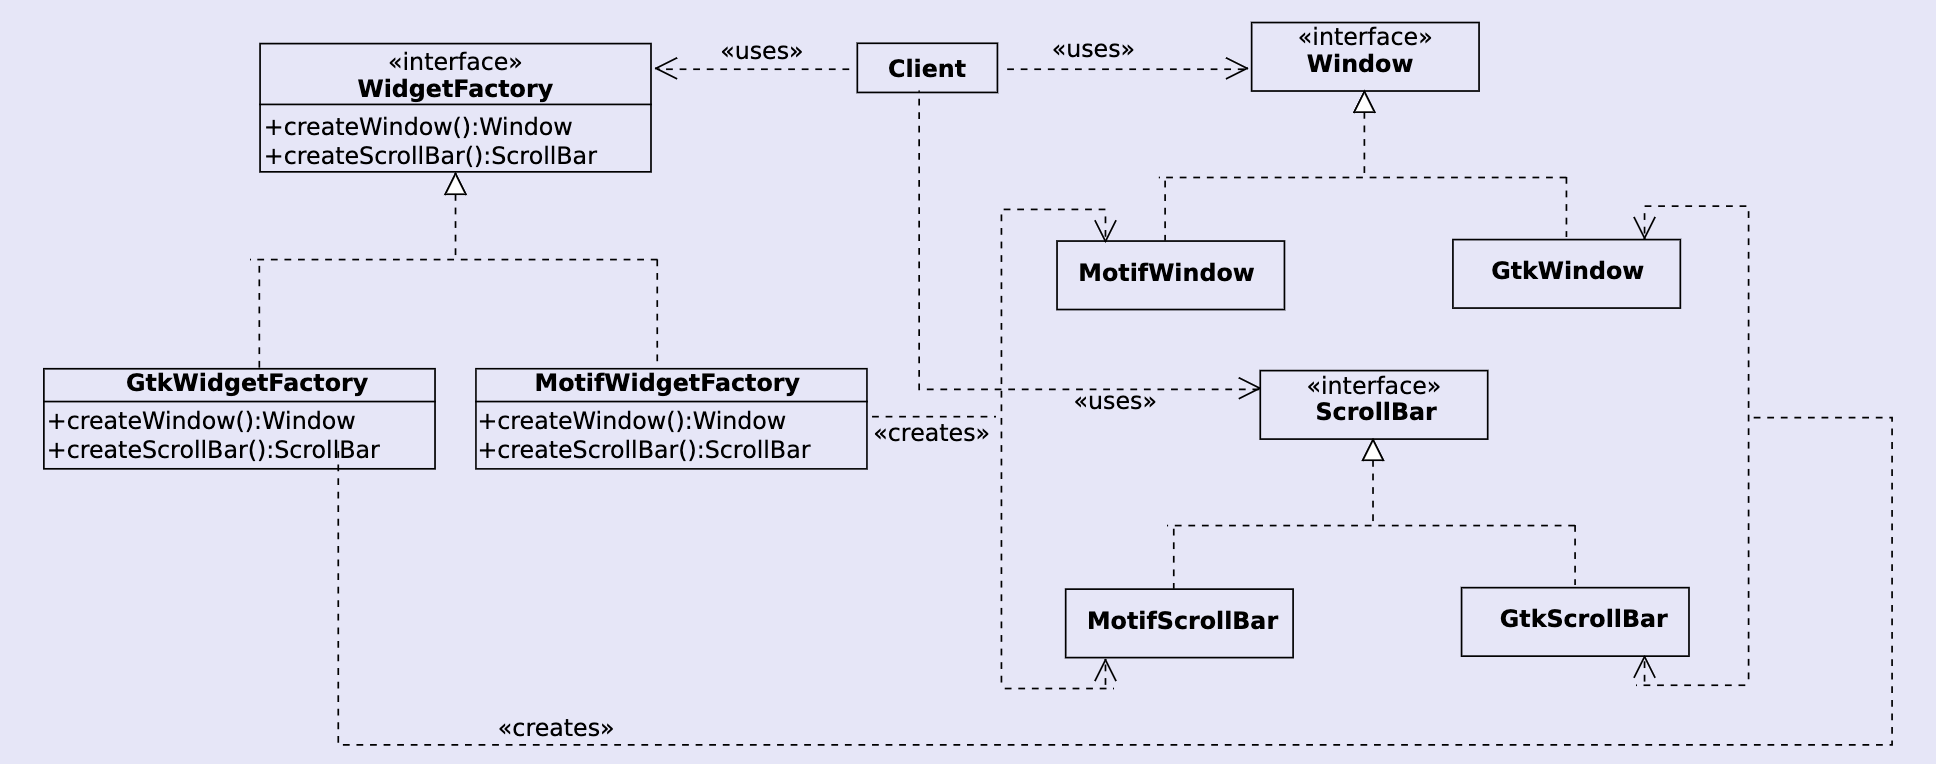
\includegraphics[width=1\linewidth]{assets/pattern/abstract-factory/abstract-factory-esempio.png}
\end{figure}

\paragraph{Soluzione} L’interfaccia WidgetFactory introduce un metodo per la creazione di ciascun tipo di base di widget definito a sua volta da un’oportuna interfaccia. I client invocano i metodi definiti da WidgetFactory per ottenere istanze di widget senza conoscere la classe concreta che utilizzano. Esiste una classe concreta che implementa WidgetFactory per ciascuno dei L\&F considerati.

\begin{figure}[H]
    \centering
    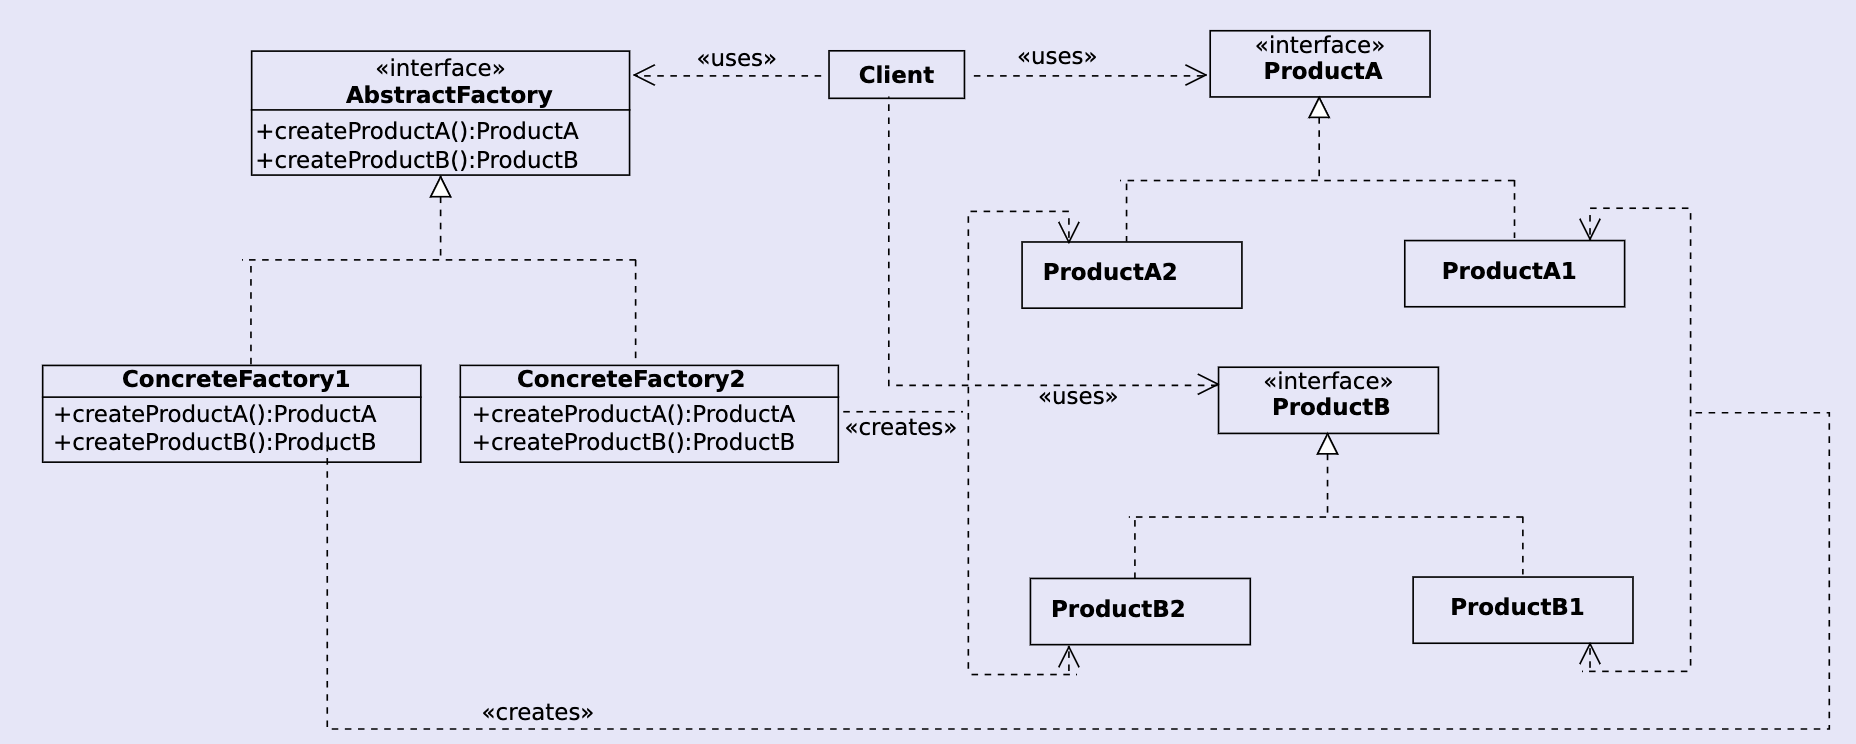
\includegraphics[width=1\linewidth]{assets/pattern/abstract-factory/abstract-factory-struttura.png}
    \caption{Class Diagram del pattern Abstract Factory}
\end{figure}

\paragraph{Struttura e Conseguenze} I partecipanti del pattern sono:
\begin{itemize}
    \item \textbf{AbstractFactory} (WidgetFactory): dichiara un’interfaccia per le operazioni di creazione di oggetti prodotto astratti.
    \item \textbf{ConcreteFactory} (MotifWidgetFactory, GtkWidgetFactory): implementa le operazioni degli oggetti prodotto concreti. 
    \item \textbf{AbstractProduct} (Window, ScrollBar): dichiara un’interfaccia per un tipo di prodotti
    \item \textbf{ConcreteProduct} (MotifWindow, GtkWindow): implementa l’interfaccia Product definendo un oggetto prodotto creato dalla corrispondente factory concreta.
\end{itemize}

Il pattern AbstractFactory consente quindi di isolare le classi concrete (processo di creazione incapsulato nella Factory), cambiare agilmente la famiglia di prodotti utilizzata (cambio di configurazione cambiando il tipo di Factory) e promuovere la coerenza nell'utilizzo dei prodotti.

È bene notare che l'aggiunta del supporto a nuove tipologie di prodotti è difficile in quanto comporta la modifica dell'interfaccia AbstractFactory e, di conseguenza, di tutte le classi che la implementano.

In più è possibile implementare il Factory come Singleton (\ref{singleton})

\begin{figure}[H]
    \centering
    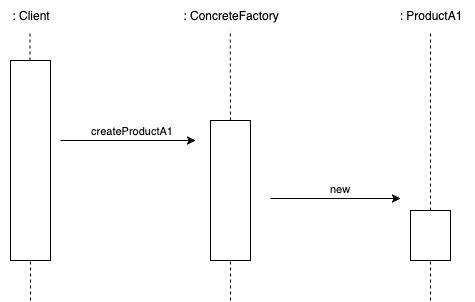
\includegraphics[width=1\linewidth]{assets/pattern/abstract-factory/abstract-factory-sequence.drawio.png}
    \caption{Sequence Diagram del pattern Abstract Factory}
\end{figure}

\newpage